\documentclass[12pt,letterpaper]{article}
\usepackage{amsmath}
\usepackage{amsfonts}
\usepackage{amsthm}
\usepackage{mathtools}
\usepackage{cancel}
\usepackage[margin=1in]{geometry}
\usepackage{titling}
\usepackage{fp}
\usepackage{enumitem}
\usepackage[super]{nth}
\usepackage{dcolumn}
\usepackage{minted}
\usepackage[title]{appendix}
\usepackage{pgfplots}
\pgfplotsset{compat=1.8}
\usepgfplotslibrary{statistics}
\usepackage[round-mode=figures,round-precision=3,scientific-notation=false]{siunitx}

\newcolumntype{d}{D{.}{.}{-1}}

\setlength{\droptitle}{-10ex}

\preauthor{\begin{flushright}\large \lineskip 0.5em}
\postauthor{\par\end{flushright}}
\predate{\begin{flushright}\large}
\postdate{\par\end{flushright}}

\title{STA 032 R Extra Credit\vspace{-2ex}}
\author{Hardy Jones\\
        999397426\\
        Professor Melcon\vspace{-2ex}}
\date{Winter 2015}

\begin{document}
  \maketitle

  \newmintedfile[rData]{r}{ fontsize=\footnotesize
                          , frame=single
                          }

  \begin{enumerate}
    \item
      \begin{enumerate}
        \item
          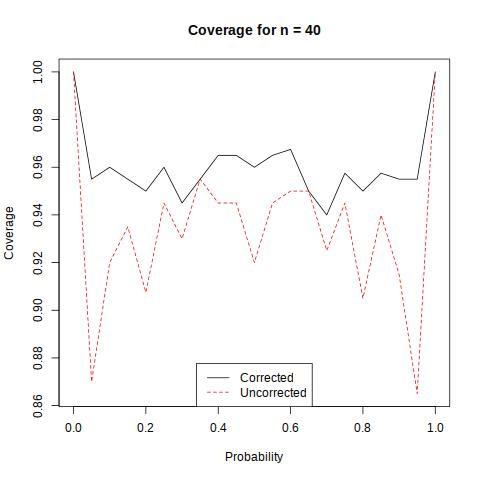
\includegraphics[width=\linewidth]{prob1a.png}
        \item
          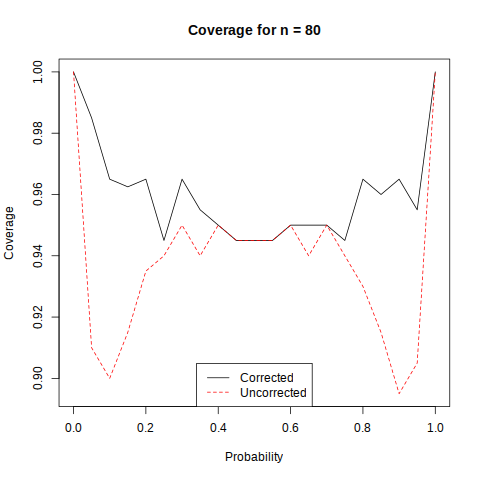
\includegraphics[width=\linewidth]{prob1b.png}
        \item
          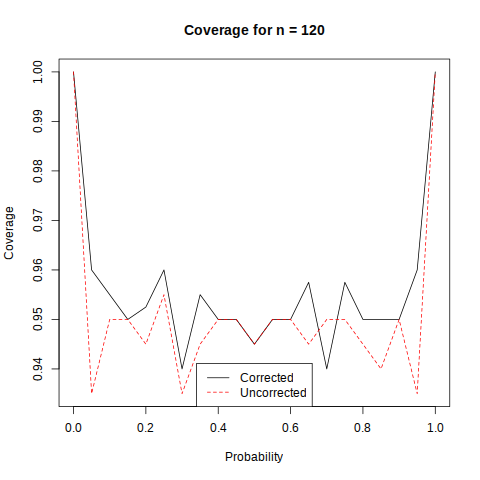
\includegraphics[width=\linewidth]{prob1c.png}
        \item
          It seems that in each simulation, the extremes of 0 and 1 give a coverage of 100\%.
          It also looks like as $n$ increases, the uncorrected confidence interval becomes better.
          The uncorrected confidence interval produces similar results for $n = 120$.
          It also seems like when $p$ is near 0.5,
          the differences between the two methods is negligible.
      \end{enumerate}
    \item
      \begin{enumerate}
        \item This student will get a score of 87.3\% for a grade of B.
        \item This student will get a score of 74.32\% for a grade of C.
        \item This student will get a score of 84.03\% for a grade of B.
        \item This student needs at least 97 points on the final for an overall score of at least 83\%.
      \end{enumerate}
  \end{enumerate}

  \begin{appendices}
    \section{R code}

        \subsection*{Problem 1}
            \rData{prob1.R}
            \subsubsection*{(a)}
                \rData{prob1a.R}
            \subsubsection*{(b)}
                \rData{prob1b.R}

        \subsection*{Problem 2}
            \rData{prob2.R}
            \subsubsection*{(a)}
                \rData{prob2a.R}
            \subsubsection*{(b)}
                \rData{prob2b.R}

        \subsection*{Problem 3}
            \rData{prob3.R}
            \subsubsection*{(a)}
                \rData{prob3a.R}
            \subsubsection*{(b)}
                \rData{prob3b.R}

\end{appendices}


\end{document}
